\documentclass{article}


\usepackage{graphicx}
\usepackage{hyperref}
\usepackage[utf8]{inputenc}
\usepackage[french]{babel}


\title{De Révolution à Evolution \\ Création d'un jeu vidéo sur les thèmes de l'écologie et de la transition énergétique}
\date{2017-2018}
\author{Niels Lachat, 3MG01 \\ Mentor : Patrick Rickli \\ Lycée Denis-de-Rougemont}

\begin{document}
        \pagenumbering{gobble}
        \maketitle
        \newpage

        \tableofcontents
        \newpage
        \pagenumbering{arabic}

        \section{Introduction}
        Le but de ce travail de maturité était de créer un jeu vidéo abordant les thématiques de l'environnement et de la transition énergétique. 
        Le genre du jeu de gestion a été choisi pour démontrer les principes économiques de la transition énergétique.
        Ces principes ont bien entendu été simplifiés et modélisés afin de pouvoir les intégrer dans un jeu vidéo.
        
        
        Je présenterai tout d'abord le concept sur lequel le jeu a été basé et j'expliquerai ensuite comment le joueur interagit avec le jeu.
        Je conclurai par une explication du fonctionnement de certaines parties du code du jeu.

        \section{Concept du jeu}
        \subsection{Développement du concept}
        
        Mon projet était de créer un jeu de gestion de ressources dont l'univers du jeu était aussi proche que possible de la réalité. Le joueur (incarnant le président/la présidente du monde fictif) commence sa partie au début du 18\textsuperscript{ème} siècle. Il devait être amené au fil des expériences du jeu à réaliser qu'à un certain moment, une transition énergétique était nécessaire afin d'assurer la survie de l'espèce humaine.
        
        
        La mécanique économique étant la mécanique principale de jeu, il était primordiale qu'elle soit bien pensée.
        Plusieurs mécaniques économiques m'ont parues intéressantes mais je n'en ai retenue qu'une seule pour les raisons décrites ci-dessous.
        
        
        La première alternative consistait à avoir deux types de centrales: des centrales produisant de l'énergie (centrales à charbon, barrages hydroélectriques, centrales nucléaires, etc...) et d'autres produisant des ressources (usines de textile, forges, champs, etc...). Le joueur installerait des centrales énergétiques pour produire de l'énergie permettant de faire fonctionner ses centrales produisant des ressources. Ainsi, un cycle économique se créerait. 
        Deux raisons m'ont convaincu de ne pas choisir cette alternative. Premièrement, l'idée ci-dessus ne transmettait pas le message que je voulais transmettre: en effet, ce n'est pas ce que l'on produit et ce que l'on consomme qui pose un problème, c'est la façon dont nous le faisons. Ce qui m'amène à la deuxième raison m'ayant fait renoncer à cette alternative: la complexité des mécaniques de jeu et par conséquent du code.
        

        \subsection{Concept final}

        \section{Le jeu}
        \subsection{Interaction du joueur}

        \subsection{Fonctionnement du jeu}
        
        \section{Conclusion}
        \subsection{Ce que j'aurais aimé rajouter dans le jeu}

        \begin{figure}[h]
                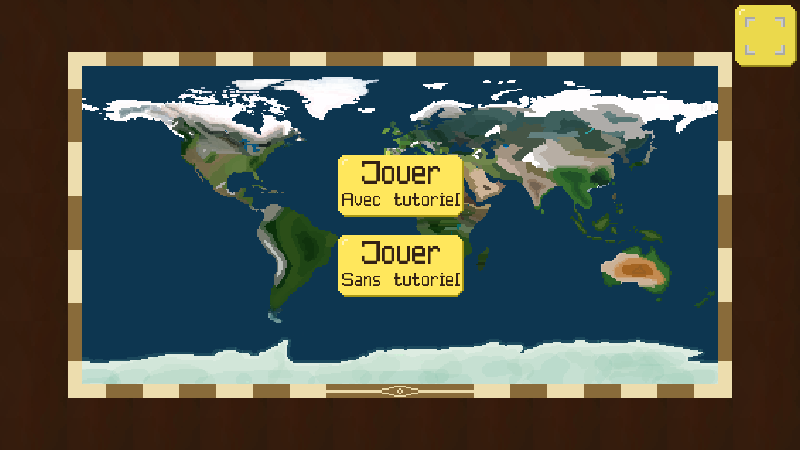
\includegraphics[width=\linewidth]{../images/mainMenu}
                \caption{Menu principal du jeu}
                \label{fig:mainMenu}
        \end{figure}

        Figure \ref{fig:mainMenu}

        \href{https://www.latex-tutorial.com/tutorials/pgfplots/}{Lien vers le tuto}



\end{document}
